% Document layout
\documentclass[a4paper,12pt]{article}
\usepackage[left=15mm, right=15mm, top=25mm, bottom=20mm]{geometry}

% \usepackage[utf8]{inputenc} % XeLaTeX doesn't need it!

% Bibliography
\usepackage[backend=biber,style=ieee]{biblatex}
\addbibresource{references.bib}

% Font
\usepackage{fontspec}
\setmainfont{TeX Gyre Termes}

% Indentation
% \setlength\parindent{0pt}
% \usepackage{indentfirst}

% Hyperlinks, Images and formatting
\usepackage[colorlinks,allcolors=black]{hyperref}
\usepackage{float}
\usepackage{graphicx}
\usepackage{multicol}
\setlength{\columnsep}{1cm}

% Section titling
\usepackage{titlesec}
%\titleformat{\section}[block]{\normalsize\textsc\filcenter}{}{0pt}{}
%\titleformat{\subsection}[block]{\normalsize\textsc\filcenter}{}{0pt}{}
\titleformat{\section}{\normalsize\scshape\filcenter}{\textnormal{\Roman{section}.}}{1em}{}

% \renewcommand{\thesection}{\Roman{section}}

% Title
\usepackage{titling}
\setlength{\droptitle}{-3em}
\title{Multiple Vessel Detection and Tracking in Harsh\\Maritime Environments}
\author{
    Nicholas Hopf\\
    up200000000
    \and
    Rodrigo Gomes\\
    up200000000
    \and
    Rui Colaço\\
    up200000000
}
\date{\vspace{-3ex}}

% Fancy header
\usepackage{fancyhdr}
\usepackage{color}
\fancypagestyle{plain}{\pagestyle{fancy}}
\thispagestyle{fancy}
\pagestyle{fancy}
\fancyhf{}
\fancyhead[R]{Computer Vision Project Report}
\fancyhead[L]{May 2023}
% \fancyfoot[L]{\textit{Faculty of Engineering - University of Porto}}
\fancyfoot[R]{Page \thepage}
\setlength{\headheight}{16pt}

%---------------------------------------------------------

\begin{document}

\maketitle


\vspace{10pt}

\begin{multicols}{2}

\textbf{{\textit{Abstract:}} This project focuses on the detection and tracking of vessels in maritime environments using computer vision techniques.
    The goal is to develop a robust tracking model for Autonomous Surface Vehicles (ASVs) that can effectively handle the challenges posed by harsh environmental conditions.
    The project leverages the research work presented in the paper titled ``Multiple Vessel Detection and Tracking in Harsh Maritime Environment''~\cite{MVDTHME} as a guide for strategies and results.
    By addressing the challenges of vessel detection and tracking in real-time and dynamic maritime scenarios, this project contributes to the advancement of computer vision research initiatives in the field of ASV navigation and collision avoidance.}
\label{tab:abstract}

\textbf{{\textit{Index Terms}}—ASV, Multiple Object Tracking, Object Detection, Computer Vision, Machine Learning, Transfer Learning, Deep Learning}
\label{tab:index}



\section{Introduction and State of the Art}\label{sec:introduction-and-state-of-the-art}
The ability of ASVs to operate autonomously in maritime environments holds great potential for applications in various domains such as surveillance, maritime transportation, and environmental monitoring.
However, the reliable detection and tracking of vessels in such environments remains a critical challenge, particularly in the presence of moving obstacles and varied lighting conditions.

To address these challenges, this project aims to develop a detection and tracking system using computer vision techniques so that an ASV is able to properly perceive neighboring vessels and move accordingly.
The work builds upon the research presented in the paper titled ``Multiple Vessel Detection and Tracking in Harsh Maritime Environment''~\cite{MVDTHME}, which provides valuable insights into strategies and results related to this specific problem domain.

The primary focus of this project is to enhance collision avoidance capabilities in ASVs by accurately detecting and tracking neighboring vessels in real-time.
The maritime environment introduces unique challenges, including multiple degrees of freedom in the observer's motion and changing lighting conditions due to harsh weather.
Therefore, the proposed tracking model needs to demonstrate robustness and reliability even in adverse conditions.

To achieve this, the project leverages transfer learning techniques based on YOLO-v8~\cite{YOLOV8}, a state-of-the-art object detection framework, for vessel detection.
Transfer learning allows the model to leverage pre-trained neural networks on large-scale datasets, significantly reducing the training time and improving performance~\cite{TRANSFERLEARNING}.
The detection module will be trained using the Singapore Maritime Dataset~\cite{SINGAPORE}, which provides videos accompanied by matrix files containing bounding box annotations for vessels in each frame.

To perform object tracking, the project employs the DeepSORT algorithm, which combines the SORT algorithm with appearance descriptors to reduce identity switches~\cite{DEEPSORT}.
DeepSORT utilizes temporal information to improve tracking accuracy and handles occlusions and temporary disappearances of vessels.
The object classifier will be trained using the Extended MARVEL Dataset~\cite{MARVEL}, which comprises a diverse collection of vessel images across 26 different classes.

PyTorch, a popular deep learning framework, will be utilized for all tasks related to neural network training, providing a flexible and efficient environment for model development and evaluation.

By developing a reliable vessel detection and tracking system, this project aims to be in line with the advancement of computer vision research initiatives in ASV navigation and collision avoidance.
The outcome will be a starting point for improving the safety and efficiency of autonomous maritime operations, with potential applications in various domains, including maritime surveillance, search and rescue, and marine transportation.

\section{Datasets}\label{sec:datasets}
The project leveraged the use of two datasets, the Extended MARVEL Dataset~\cite{MARVEL} and the Singapore Maritime Dataset~\cite{SINGAPORE}.

The MARVEL Dataset is a comprehensive collection of images prepared for training the classifier in the tracking module.
The dataset consists of a vast repository of 138,367 images showcasing different vessels from various viewpoints and perspectives.
The images are carefully distributed over 26 distinct vessel classes, representing a wide range of maritime vessels, including cargo ships, fishing boats and sailboats.
The dataset provides a rich variety of vessel types, enabling the development of a highly accurate and robust classifier.

The Singapore Maritime Dataset encompasses a collection of videos that were used for training and evaluating the object detection process.
The dataset provides realistic vessel observations, in both onshore and onboard scenarios, capturing the complexity and challenges of real-world maritime operations.
The 81 videos, which, in total, have a size of 5278 Mb, encompass diverse lighting conditions, vessel types, and dynamic movements, making it a valuable resource for developing robust detection algorithms.
Each video in the dataset is accompanied by matrix files that contain bounding box annotations for every object present in each frame.
By leveraging this data, the project aims to improve the vessel detection step, enhancing the overall performance and reliability of the system.

\section{Methodology}\label{sec:methodology}
Our objective was to replicate and experiment with the techniques adopted in the original paper~\cite{MVDTHME}, making it possible to accurately track multiple vessels in real-time from a video feed captured by an onboard camera.

To achieve such result, the final algorithm was divided in three steps:
\begin{enumerate}
    \item \textbf{Detect} vessels from each frame with YOLO~\cite{YOLOV8}, computing their bounding boxes
    \item \textbf{Classify} each detected object with YOLO~\cite{YOLOV8} considering the 26 vessel classes from the MARVEL dataset
    \item \textbf{Track} the detected vessels with DeepSORT~\cite{DEEPSORT} given the detection result for each frame
    \item \textbf{Draw} the tracking ID and the bounding box for each vessel in the input video for a qualitative evaluation of the system
\end{enumerate}

To train the vessel detection model we obtained one image for every 0.5 seconds in each video from the Singapore Maritime Dataset~\cite{SINGAPORE}, where training and validation images were divided using a 9:1 ratio.
Then, the YOLO-v8 ``nano'' detection model was used with its pre-trained weights, so the performed training process benefits from a transfer learning approach.

Beyond the common augmentation techniques already included in the YOLO training process, we also tried performing histogram correction and sharpening to augment the data and minimize exposure issues that are sometimes present in the images, although our best trained model was achieved without the inclusion of histogram corrected images.

Based on the successful results of the original paper~\cite{MVDTHME}, the Adaptive Moment Estimation (Adam) optimizer was chosen for the object detection training process.
The evaluation metric used in this study is Mean Average Precision (mAP), which serves as a measure to compare the accuracy of different training exercises.
The mAP calculation involves assessing the precision of detections for each class of objects in the dataset.
Initially, the focus is on mAP with an Intersection over Union (IoU) threshold of more than 50\%.
This threshold determines the overlap between predicted bounding boxes and ground truth boxes.
By calculating the average precision at this IoU threshold, the performance of the models can be evaluated based on their ability to accurately detect objects.

The Extended MARVEL Dataset~\cite{MARVEL} was used to train the image classifier, while the Stochastic Gradient Descent (SGD) optimizer was used during the training process that ran during 20 epochs.
Since the MARVEL dataset has a considerably large number of images for each vessel class, the training and validation images were divided using an 8:2 ratio.
Then, the YOLO-v8 ``small'' classification model was used with its pre-trained weights, so the performed training process benefits from a transfer learning approach.

\section{Results and Analysis}\label{sec:results-and-analysis}

Since the training data for the vessel detection model was limited, the best results were achieved by grouping all images into a single ``boat'' class, that encompasses all vessels that should be detected by YOLO\@.

The Precision-Recall results demonstrate that, although there is a non-negligible occurrence of false positives, the overall effectiveness of the detector is still significant.

\begin{figure}[H]
    \centering
    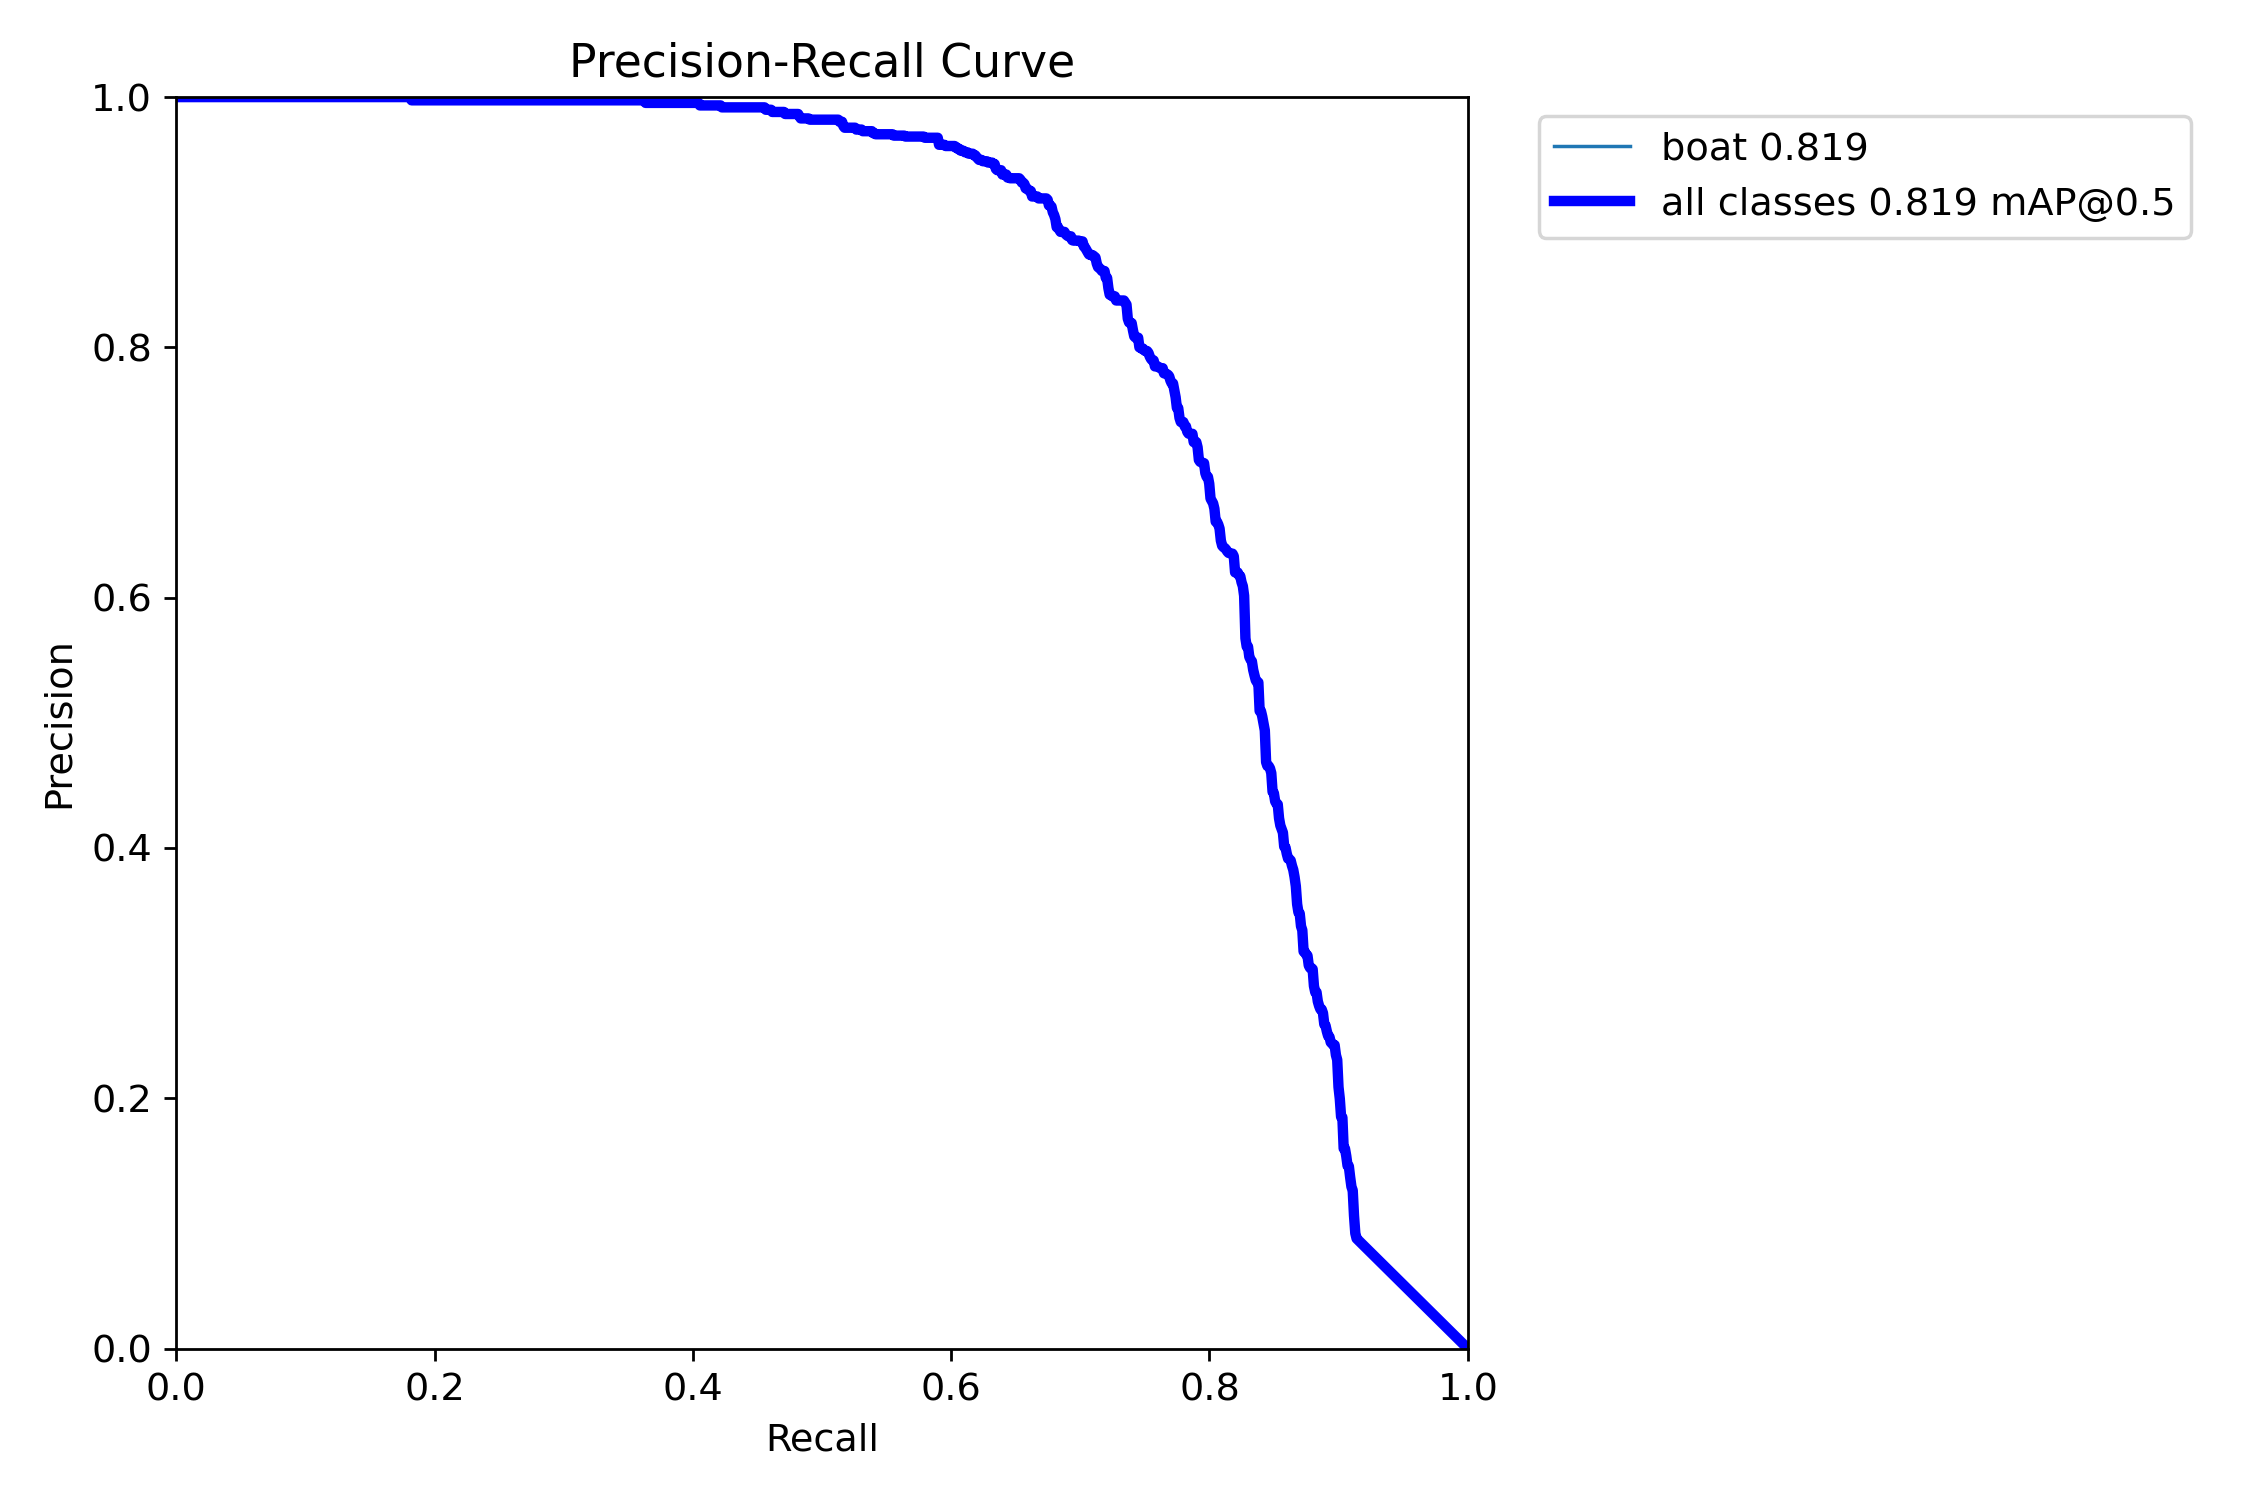
\includegraphics[width=0.45\textwidth]{images/detection/PR_curve}
    \caption{Vessel detection precision-recall Curve}
    \label{fig:1}
\end{figure}

Due to hardware limitations, the ``nano'' detection model of YOLO-v8, that has 3.2 million parameters, was used for training during 20 epochs.
Even with a small number of parameters, we are able to observe an effective optimization during the training of the detector.

\begin{figure}[H]
    \centering
    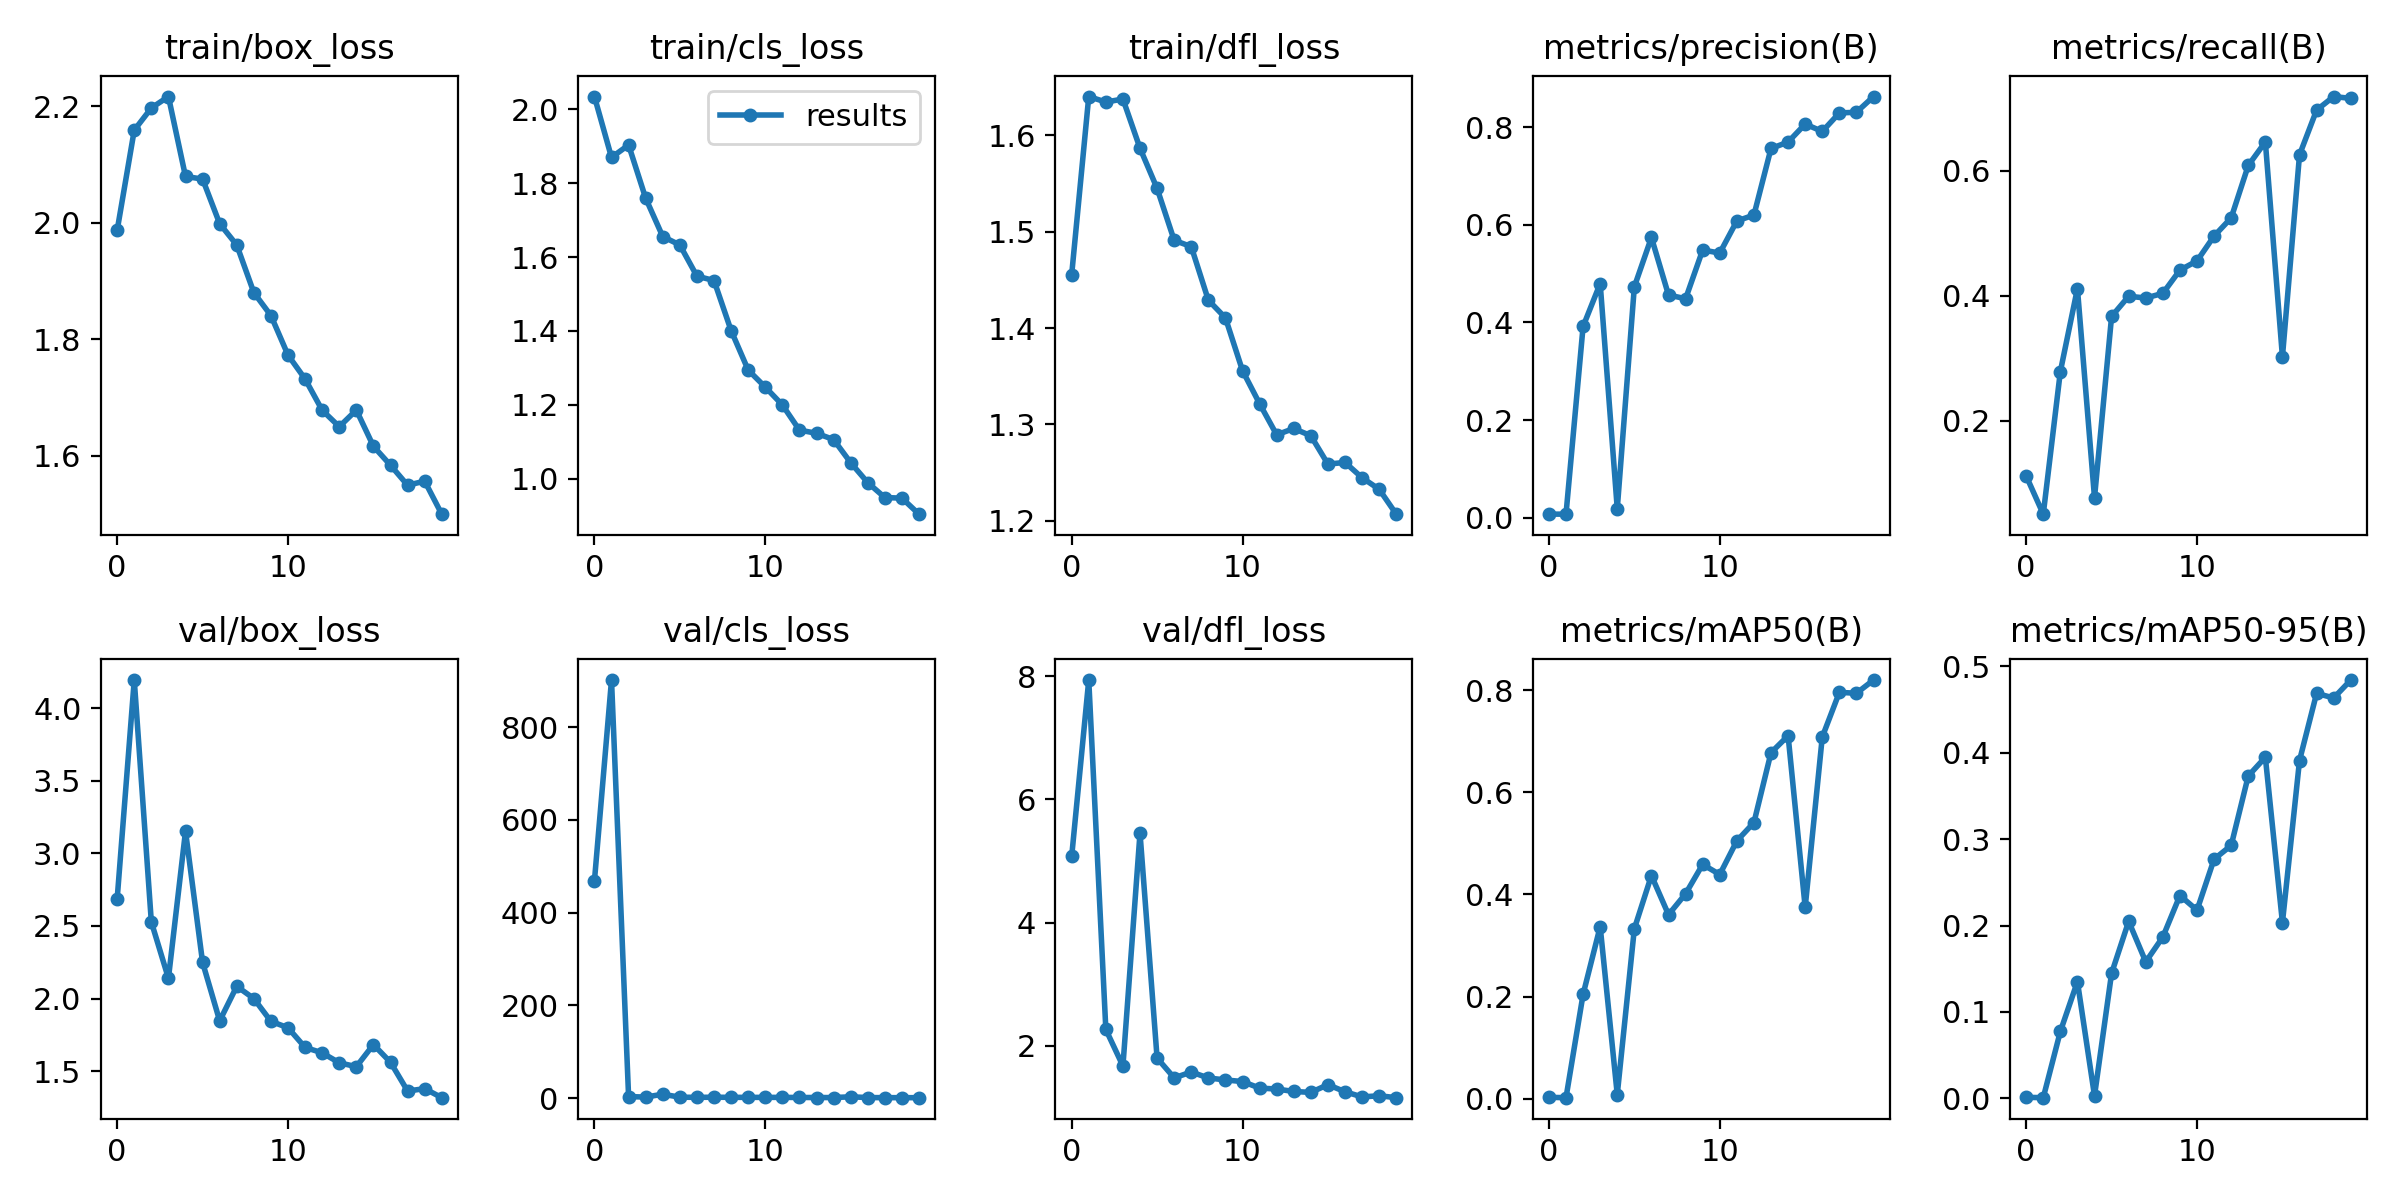
\includegraphics[width=0.45\textwidth]{images/detection/detection_results}
    \caption{Vessel detection training metrics}
    \label{fig:2}
\end{figure}

The classification loss for the validation dataset has a rapid descent to zero since the model learns that there is only a single class, so its value is always deterministic.

After training, it is possible to verify the qualitative detection results by using YOLO with the trained model and predicting the class and bounding boxes of objects in randomly selected frames from the validation video dataset.

\begin{figure}[H]
    \centering
    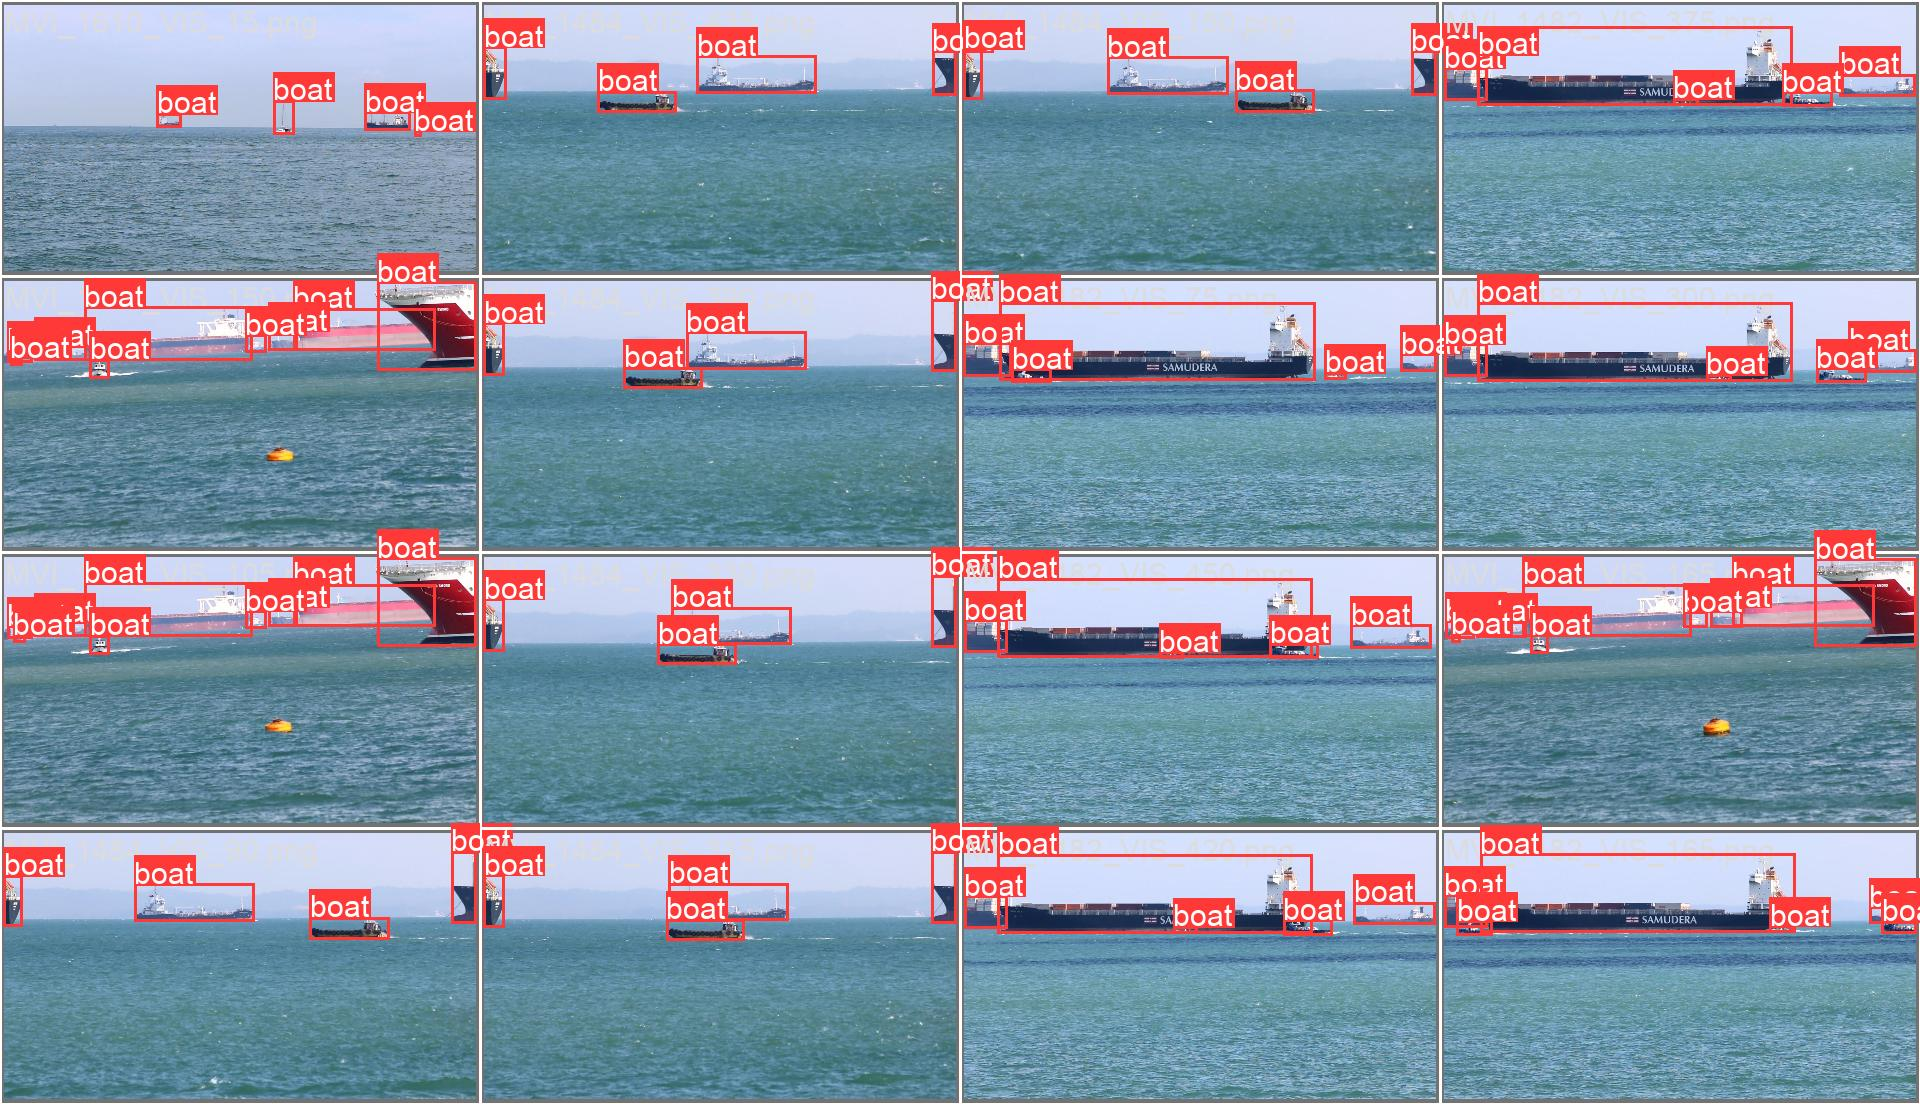
\includegraphics[width=0.45\textwidth]{images/detection/validation_labels}
    \caption{Vessel detection validation examples}
    \label{fig:3}
\end{figure}

The detection results were perceptibly favorable, as the detector was able to properly identify varied and distant vessels, and even differentiate overlapping ships.

Then, after successfully training the object detection model, the next step was training the classification model.
Since this training process resorted to the ``small'' classification model of YOLO-v8, that has 6.4 million parameters and had an extensive dataset to be trained on, the results were optimal.

\begin{figure}[H]
    \centering
    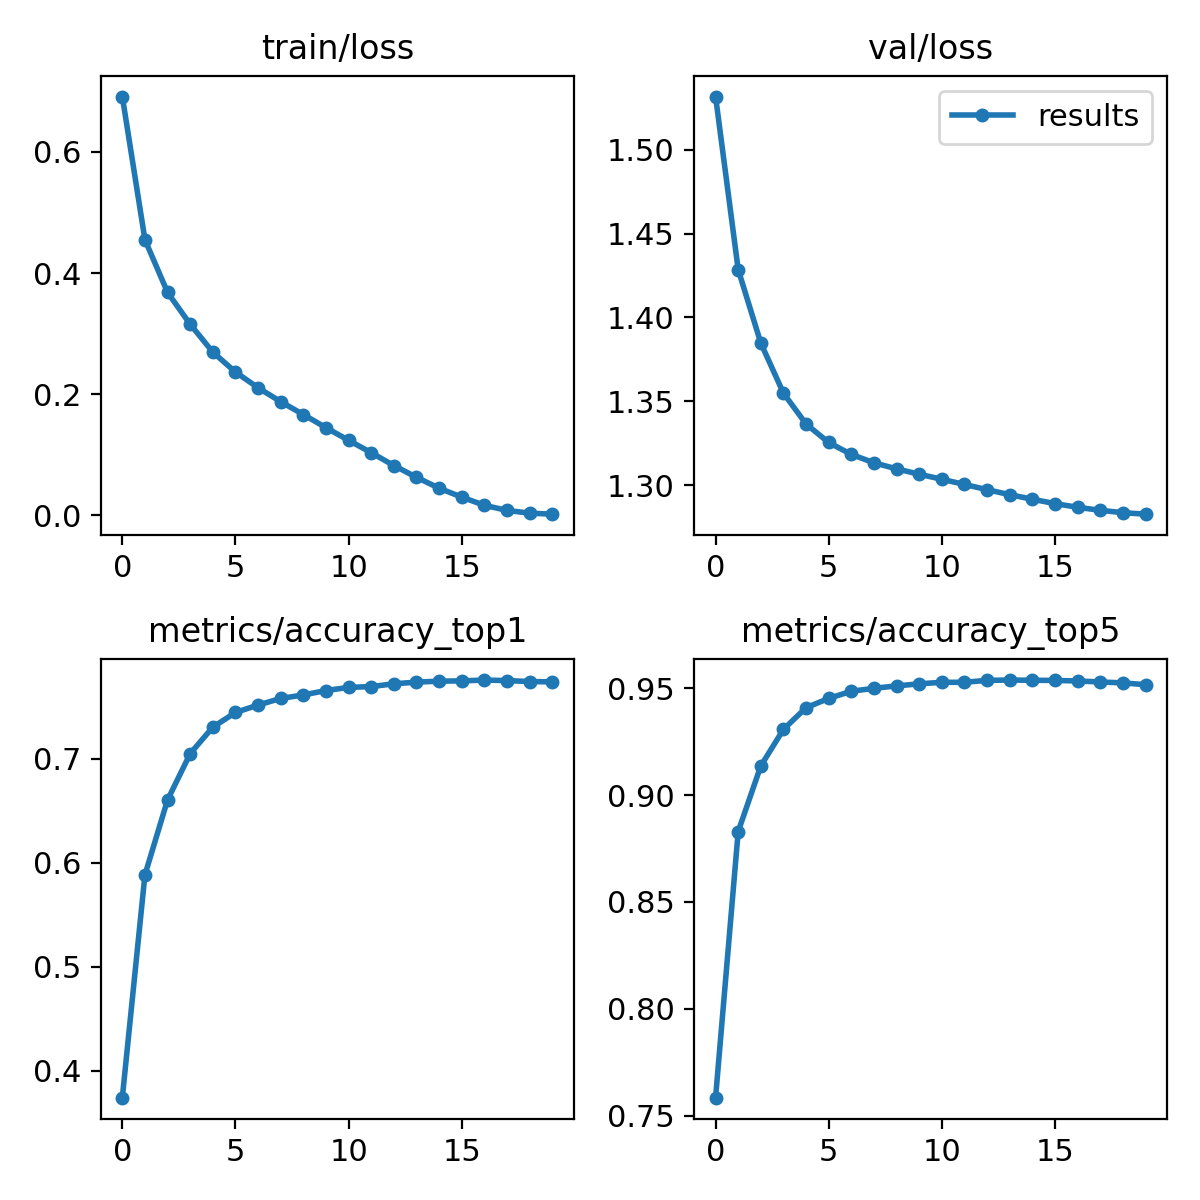
\includegraphics[width=0.45\textwidth]{images/classification/classification_results}
    \caption{Vessel classification training metrics}
    \label{fig:4}
\end{figure}

After 20 training epochs, it is possible to verify that the model converged.
This implies that the classification confidence is above 70\% for most vessel classes, as evident in the confusion matrix.

\begin{figure}[H]
    \centering
    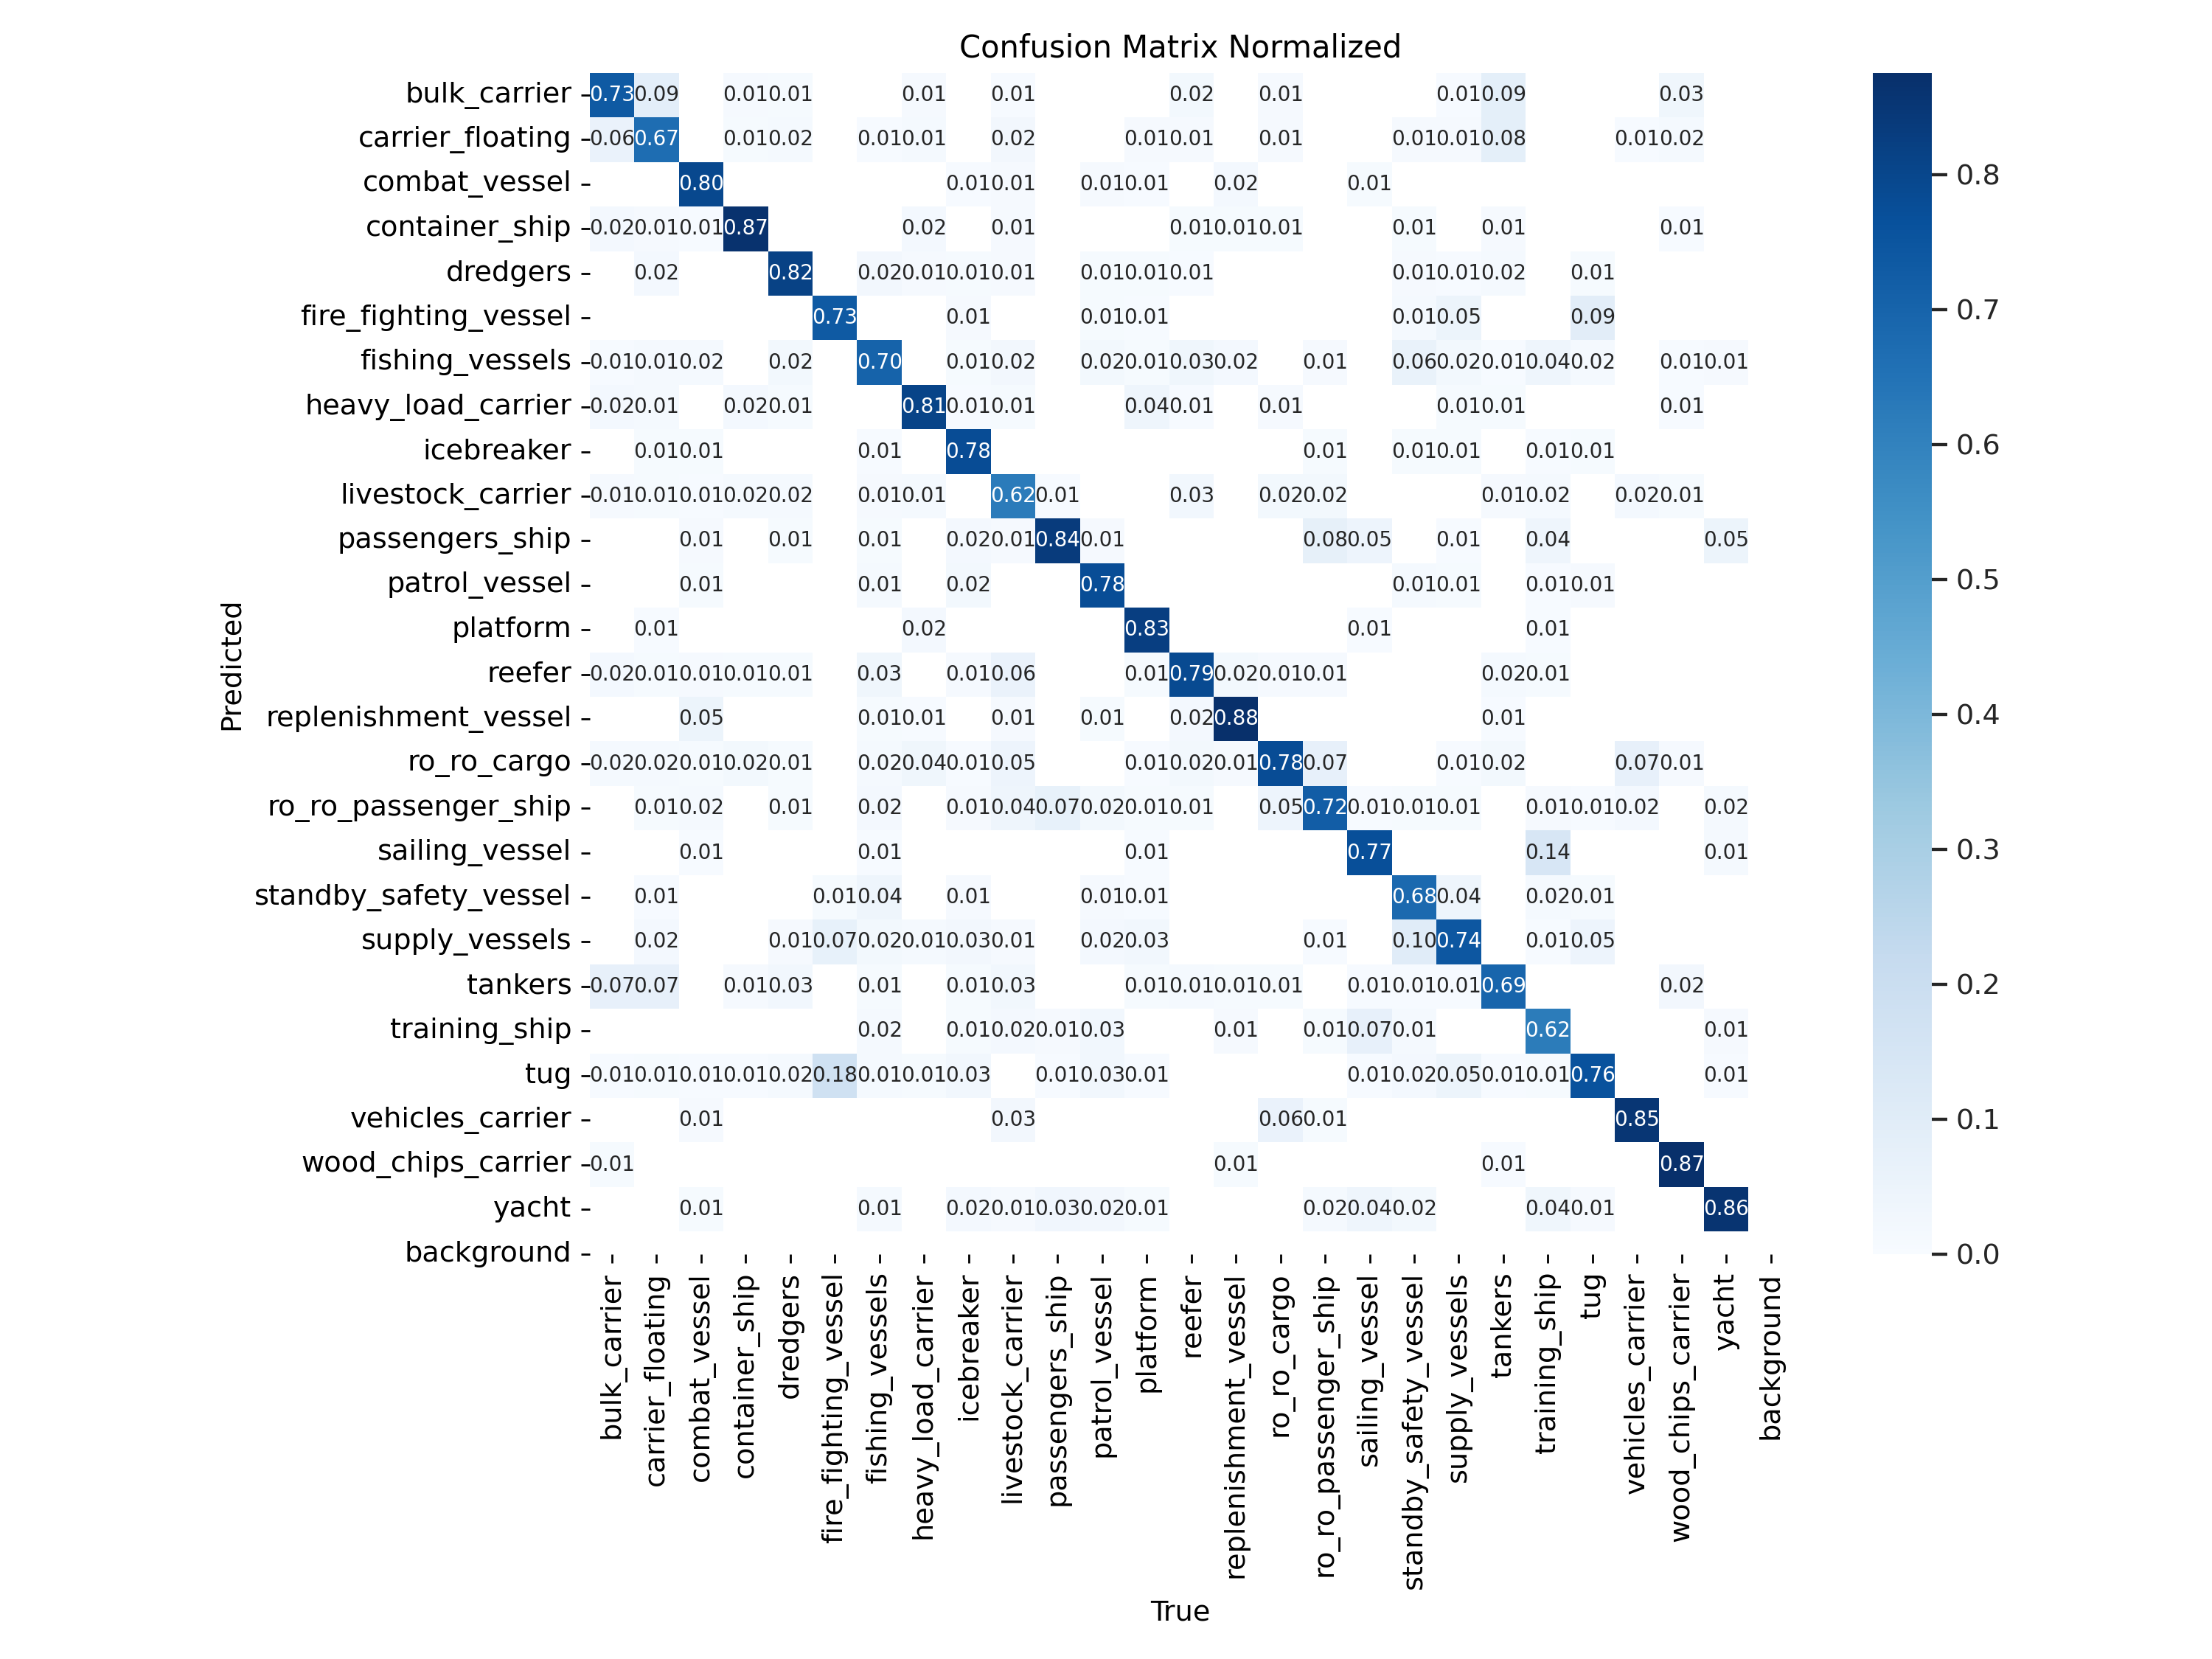
\includegraphics[width=0.45\textwidth]{images/classification/confusion_matrix_normalized}
    \caption{Vessel classification confusion matrix}
    \label{fig:5}
\end{figure}

Depending on the application it is possible to group similar vessel classes, such as the 3 categories of sail boats, thus improving the overall prediction confidence of the model.
After training, it is possible to verify the qualitative classification results by using YOLO with the trained model and predicting the class of randomly selected images from the validation dataset.

\begin{figure}[H]
    \centering
    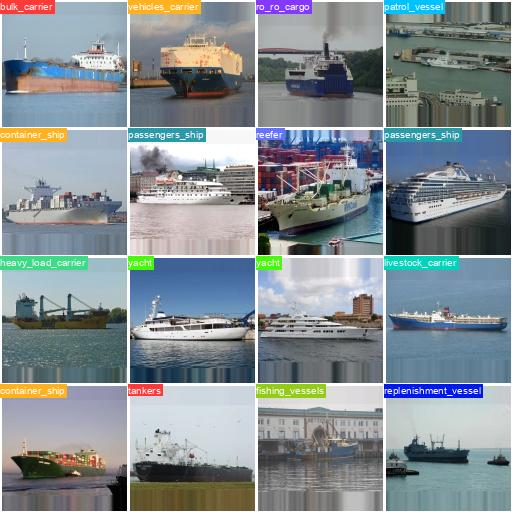
\includegraphics[width=0.45\textwidth]{images/classification/validation_labels}
    \caption{Vessel classification validation examples}
    \label{fig:6}
\end{figure}

After concluding the detection and classification training phases, the tracking step was implemented.
Considering only the vessels detected by YOLO with a confidence value greater than the threshold (0.7), the detection information is sent to DeepSORT, which returns the ID of the tracked object and its resulting bounding box after compensating problems such as occlusion with solutions such as the Kalman filter.

Most vessels are properly tracked, although distant boats tend to have a detection confidence lower than the threshold, it is still a viable solution for maneuvering an ASVs based on the closest neighboring vessels.

\begin{figure}[H]
    \centering
    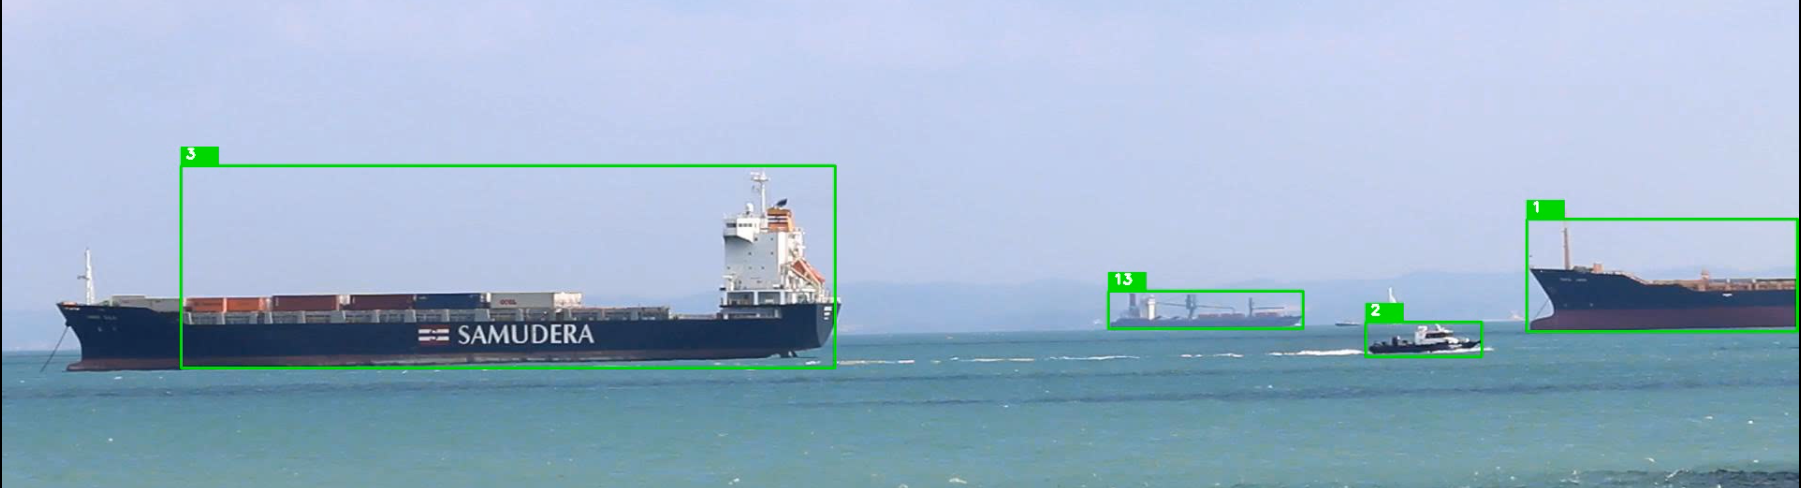
\includegraphics[width=0.45\textwidth]{images/tracking/detected_ships}
    \caption{Multiple vessel tracking}
    \label{fig:7}
\end{figure}

Even in onboard situations, where the camera executes sharp movements and has slight changes in focus, the tracking is still effective.

\begin{figure}[H]
    \centering
    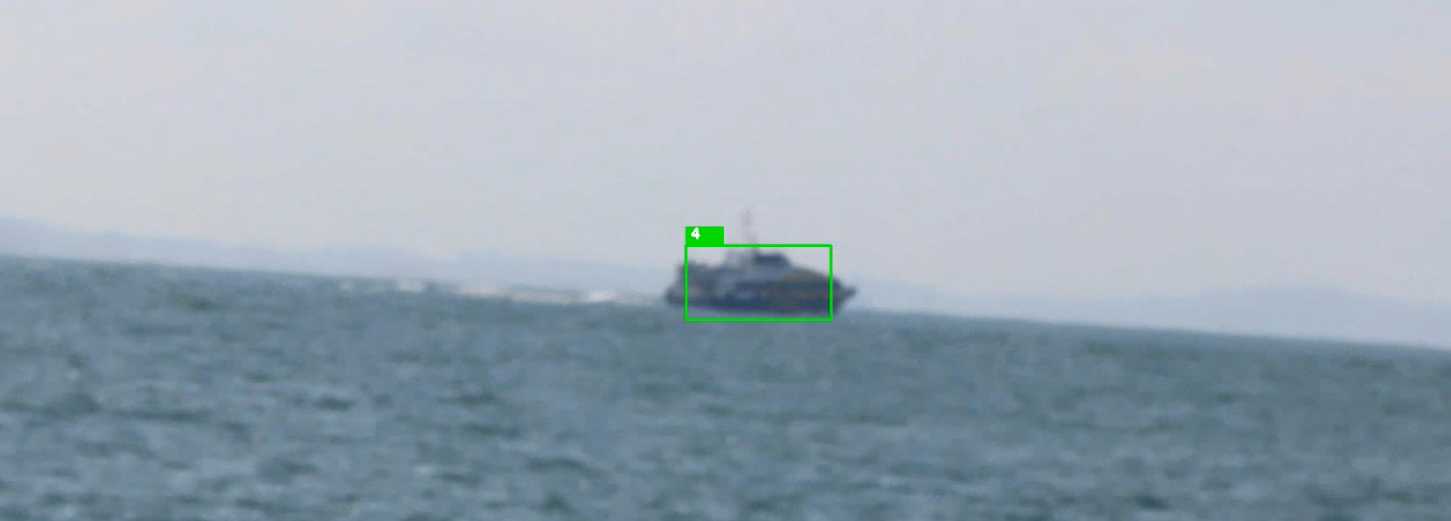
\includegraphics[width=0.45\textwidth]{images/tracking/blurred_ship}
    \caption{Tracking with heavy camera motion and blurring}
    \label{fig:8}
\end{figure}

Furthermore, tracking on a Full HD video feed had a consistent average of 10 frames per second on tests performed locally on an 8-year-old laptop, demonstrating that real-time tracking is viable with the implemented algorithms if they were to be used in a dedicated machine.

\section{Opportunities}\label{sec:opportunities}
Some cases of incorrect labeling due to anchor overlapping (object occlusion) were identified in the implementation described above, although DeepSORT should be resilient against such situations.
To solve this issue, it is possible to perform ``Non-Maximum Suppression'' or change the applied method, resorting to an anchor-free tracking approach.
In March 2023 Yantong \textit{et al.}~\cite{FAIRMOT} obtained successful tracking results with the Singapore Maritime Dataset while working with FairMOT and Deep Layer Aggregation (DLA) instead of DeepSORT and YOLO\@.
Another option for exploration would be resorting to the recently published StrongSORT~\cite{STRONGSORT} tracker.

\section{References}\label{sec:references}
\printbibliography[heading=none]
\end{multicols}
\end{document}
